\documentclass[11pt, a4paper]{article}
\usepackage[english]{babel}
\usepackage{hyperref}
\usepackage{graphicx}
\usepackage{amsmath}
\usepackage{amssymb}
\usepackage{tabularx}
% LaTeX settings for MATLAB code listings
% based on Ted Pavlic's settings in http://links.tedpavlic.com/ascii/homework_new_tex.ascii
\usepackage{listings}
\usepackage[usenames,dvipsnames]{color}

% This is the color used for MATLAB comments below
\definecolor{MyDarkGreen}{rgb}{0.0,0.4,0.0}

% For faster processing, load Matlab syntax for listings
\lstloadlanguages{Matlab}%
\lstset{language=Matlab,                        % Use MATLAB
    	breakindent=40pt, 
   		breaklines,
        frame=single,                           % Single frame around code
        basicstyle=\small\ttfamily,             % Use small true type font
%		basicstyle=\footnotesize,
        keywordstyle=[1]\color{Blue}\bfseries,  % MATLAB functions bold and blue
        keywordstyle=[2]\color{Purple},         % MATLAB function arguments purple
        keywordstyle=[3]\color{Blue}\underbar,  % User functions underlined and blue
        identifierstyle=,                       % Nothing special about identifiers
                                                % Comments small dark green courier
        commentstyle=\usefont{T1}{pcr}{m}{sl}\color{MyDarkGreen}\small,
        stringstyle=\color{Purple},             % Strings are purple
        showstringspaces=false,                 % Don't put marks in string spaces
        tabsize=4,                              % 5 spaces per tab
        %
        %%% Put standard MATLAB functions not included in the default
        %%% language here
        morekeywords={xlim,ylim,var,alpha,factorial,poissrnd,normpdf,normcdf,specifyCoefficients},
        %
        %%% Put MATLAB function parameters here
        morekeywords=[2]{on, off, interp},
        %
        %%% Put user defined functions here
        morekeywords=[3]{FindESS, homework_example},
        %
        morecomment=[l][\color{Blue}]{...},     % Line continuation (...) like blue comment
        numbers=left,                           % Line numbers on left
        firstnumber=1,                          % Line numbers start with line 1
        numberstyle=\tiny\color{Blue},          % Line numbers are blue
        stepnumber=1                            % Line numbers go in steps of 5
        }

% Includes a MATLAB script.
% The first parameter is the label, which also is the name of the script
%   without the .m.
% The second parameter is the optional caption.
\newcommand{\matlabscript}[2]
  {\begin{itemize}\item[]\lstinputlisting[caption=#2,label=#1]{#1.m}\end{itemize}}

\title{2D Poisson equation}
\author{Gilbert Fran\c cois Duivesteijn}

\begin{document}
\maketitle

\begin{figure}
  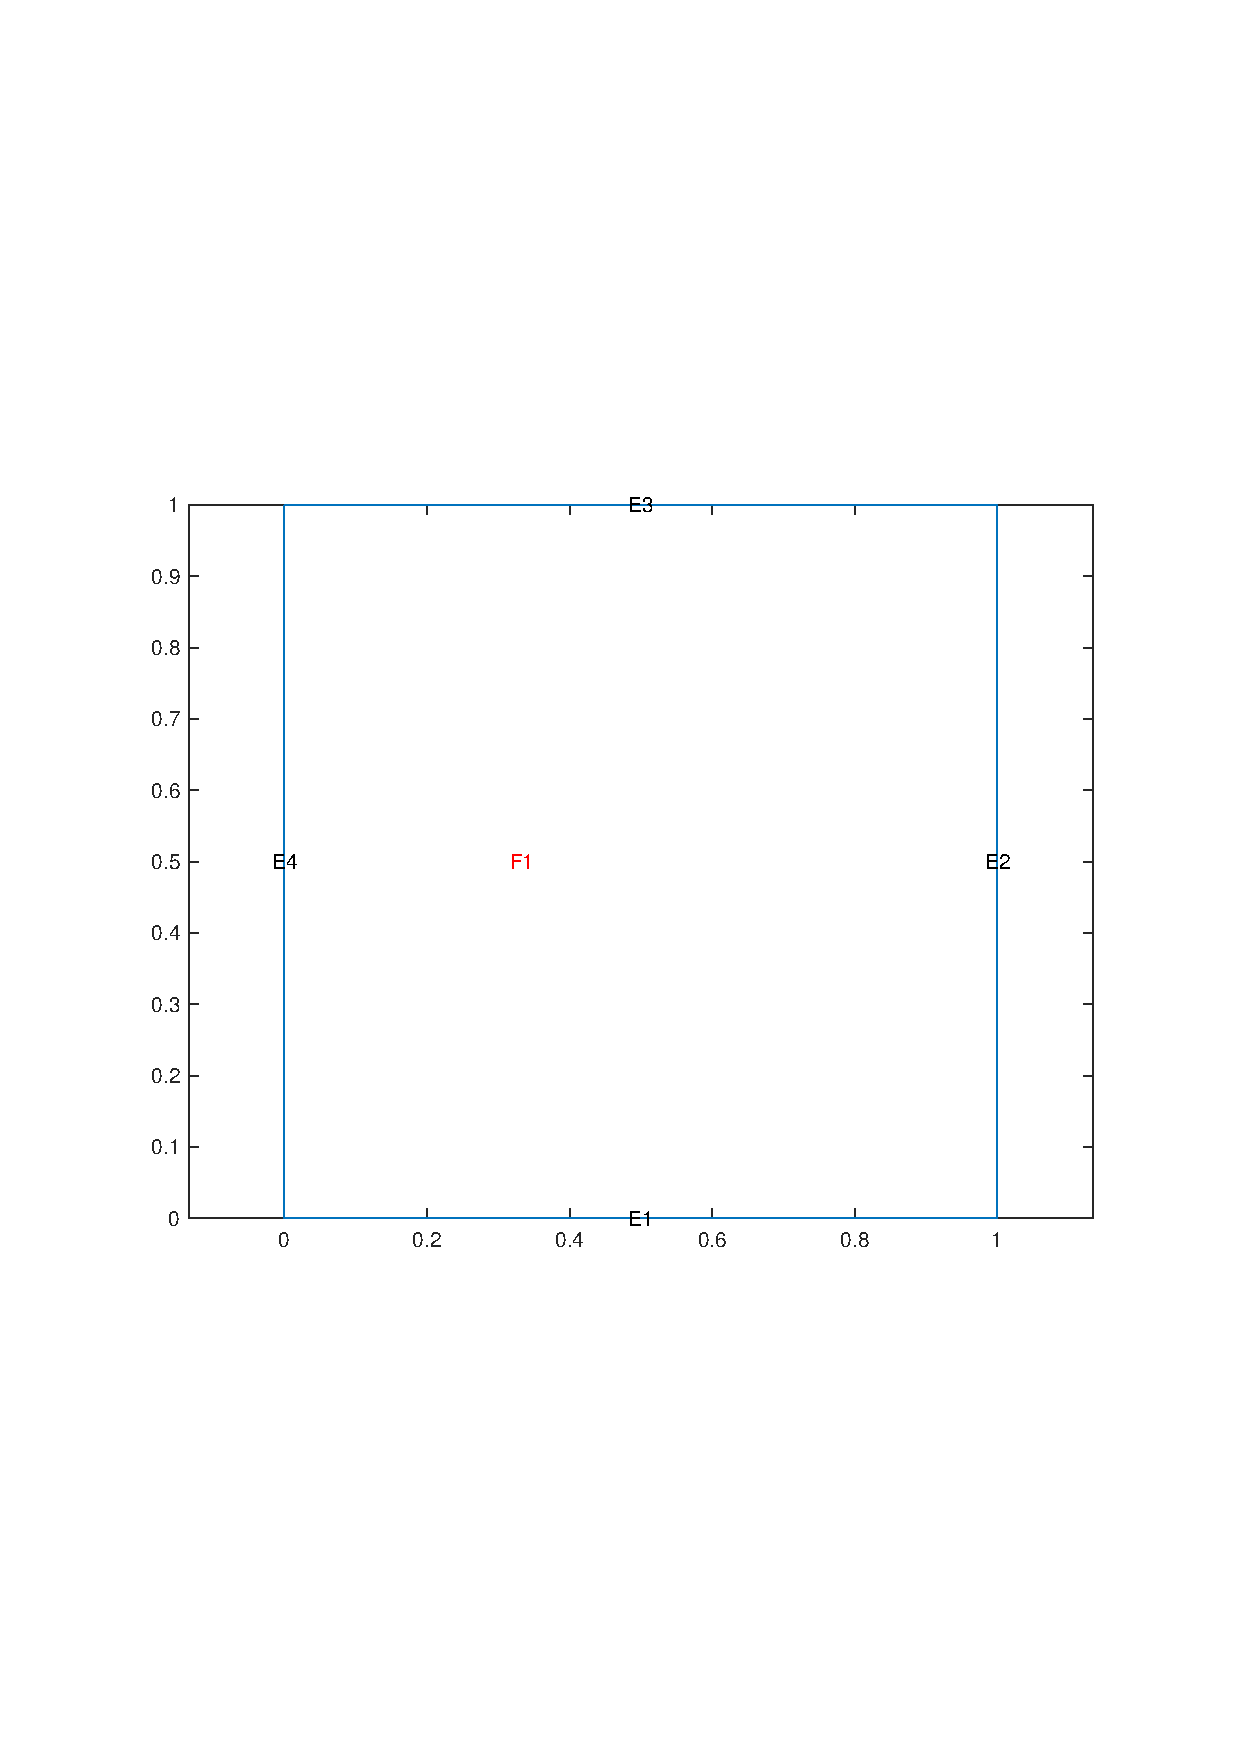
\includegraphics[width=0.49\textwidth]{assets/domain.pdf}
  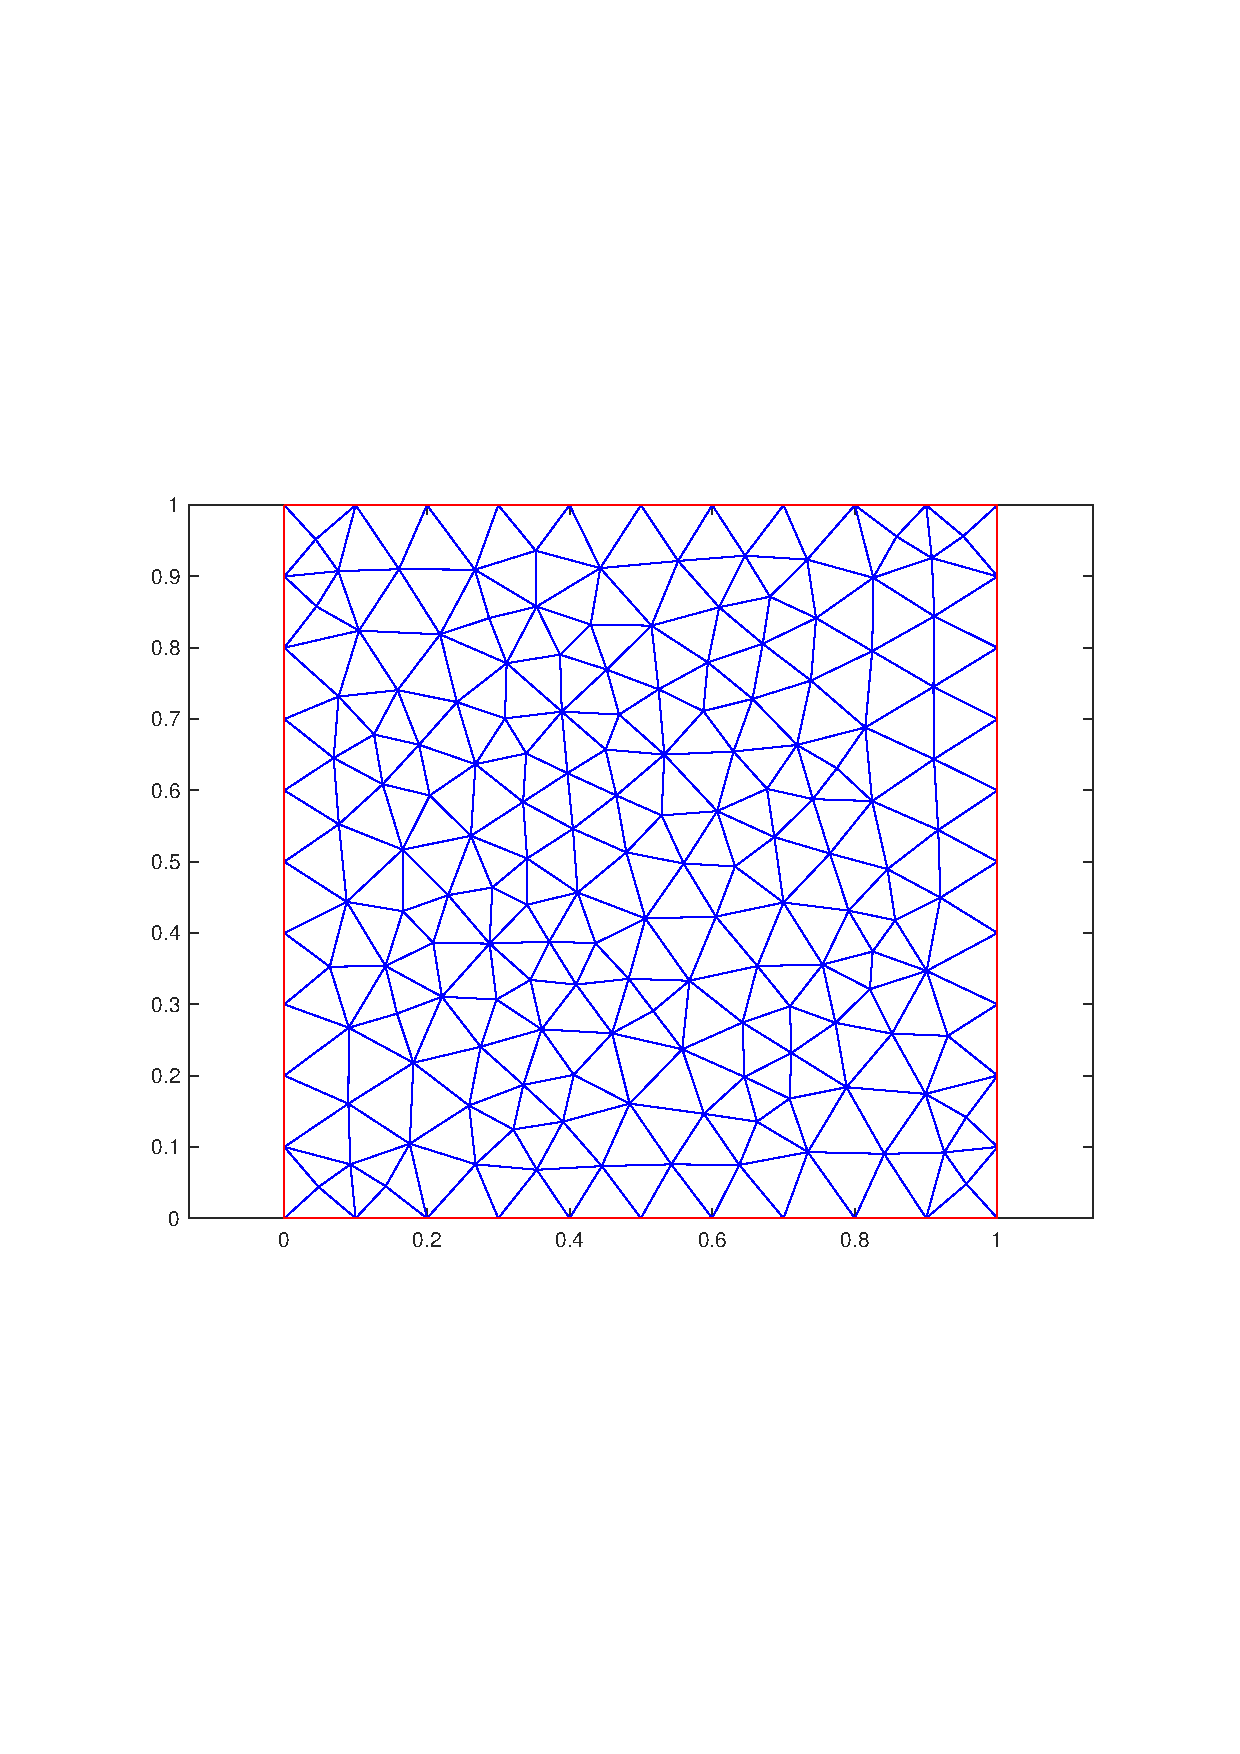
\includegraphics[width=0.49\textwidth]{assets/mesh.pdf}
  \caption{Computational domain with edge and face labels (left). Unstructured grid (right).}\label{fig:domain}
\end{figure}

This Matlab implementation is for verification and validation for the python code ``2D Poisson equation, finite difference''. The Matlab PDE Toolbox v2017a is used. The Jupyter Notebook is located at \href{https://github.com/gilbertfrancois/partial-differential-equations/blob/ffee191364d9a2417bef08f517cab05114de68c5/notebook/2D%20Poisson%20equation,%20finite%20difference.ipynb}{[1]}. Let's analyse the domain on the unit square (figure \ref{fig:domain}) and solve the 2D Poisson equation 
\begin{align}
\kappa \nabla^2 u + f = 0\label{eq:pde}
\end{align}
with
\begin{align}
f(x, y) &= -\sin(x)\cos(y),
\end{align}
boundary conditions
\begin{align}
u &= 0 \qquad \textrm{on} \quad [E_1, E_2, E_3, E_4] \label{eq:bc1}\\
\end{align}
and initial condition
\begin{align}
u(t=0) &= 0	\qquad \textrm{on} \quad F_1 \label{eq:init}
\end{align}


Matlab has a generic PDE formula that you can tune to your problem by setting the coefficients. The solvepde function models the equation:
\begin{align}
m\frac{\partial^2 u}{\partial t^2} + d\frac{\partial u}{\partial t} - \nabla \cdot (c\nabla u) + au &= f \label{eq:pde_ref}	
\end{align}
The coefficients to set are $m$, $d$, $c$, $a$ and $f$. To define (\ref{eq:pde}), we set $m=0$, $d=1$, $c=\kappa$, $a=0$ and $f=@fn\_fxy$.

\begin{lstlisting}[language=Matlab]
%% Specify the PDE model
specifyCoefficients(    ...
    model,              ...
    'm', 0,             ...
    'd', 1,             ...
    'c', 1,             ...
    'a', 0,             ...
    'f', @fn_fxy        ...
);
\end{lstlisting}
The function \texttt{fn\_fxy} is implemented in a separate file

\begin{lstlisting}[language=Matlab]
%% file: fn_fxy.m
function f = fn_fxy( location, state )
    f(1,:) = -sin(location.x) .* cos(location.y);
end
\end{lstlisting}

The Dirichlet boundary condition implies that the solution u on a particular edge or face satisfies the equation
\begin{align}
	hu = r
\end{align}
where $h$ and $r$ are functions defined on $\partial \Omega$. The boundary conditions from (\ref{eq:bc1}) can be constructed by specifying $u=0$:

\begin{lstlisting}[language=Matlab]
%% Boundary conditions
applyBoundaryCondition(model,           ...
    'dirichlet', 						...
    'edge', [1, 2, 3, 4],        				...
    'u', 0);
	
\end{lstlisting}

Let's set the initial condition from equation (\ref{eq:init}) by creating a function and reference the function pointer in the function setInitialConditions.

\begin{lstlisting}[language=Matlab]
%% Initial conditions.
setInitialConditions(model, @fn_u0);
\end{lstlisting}


Generate the mesh, solve the PDE and get the results from the result object:
\begin{lstlisting}[language=Matlab]
%% Generate mesh.
generateMesh(model, 'Hmax', 0.1);

%% Time domain
t = 0:0.01:10;

%% Solve the PDE
result = solvepde(model, t);
u = result.NodalSolution;
\end{lstlisting}

\begin{figure}[htb]
  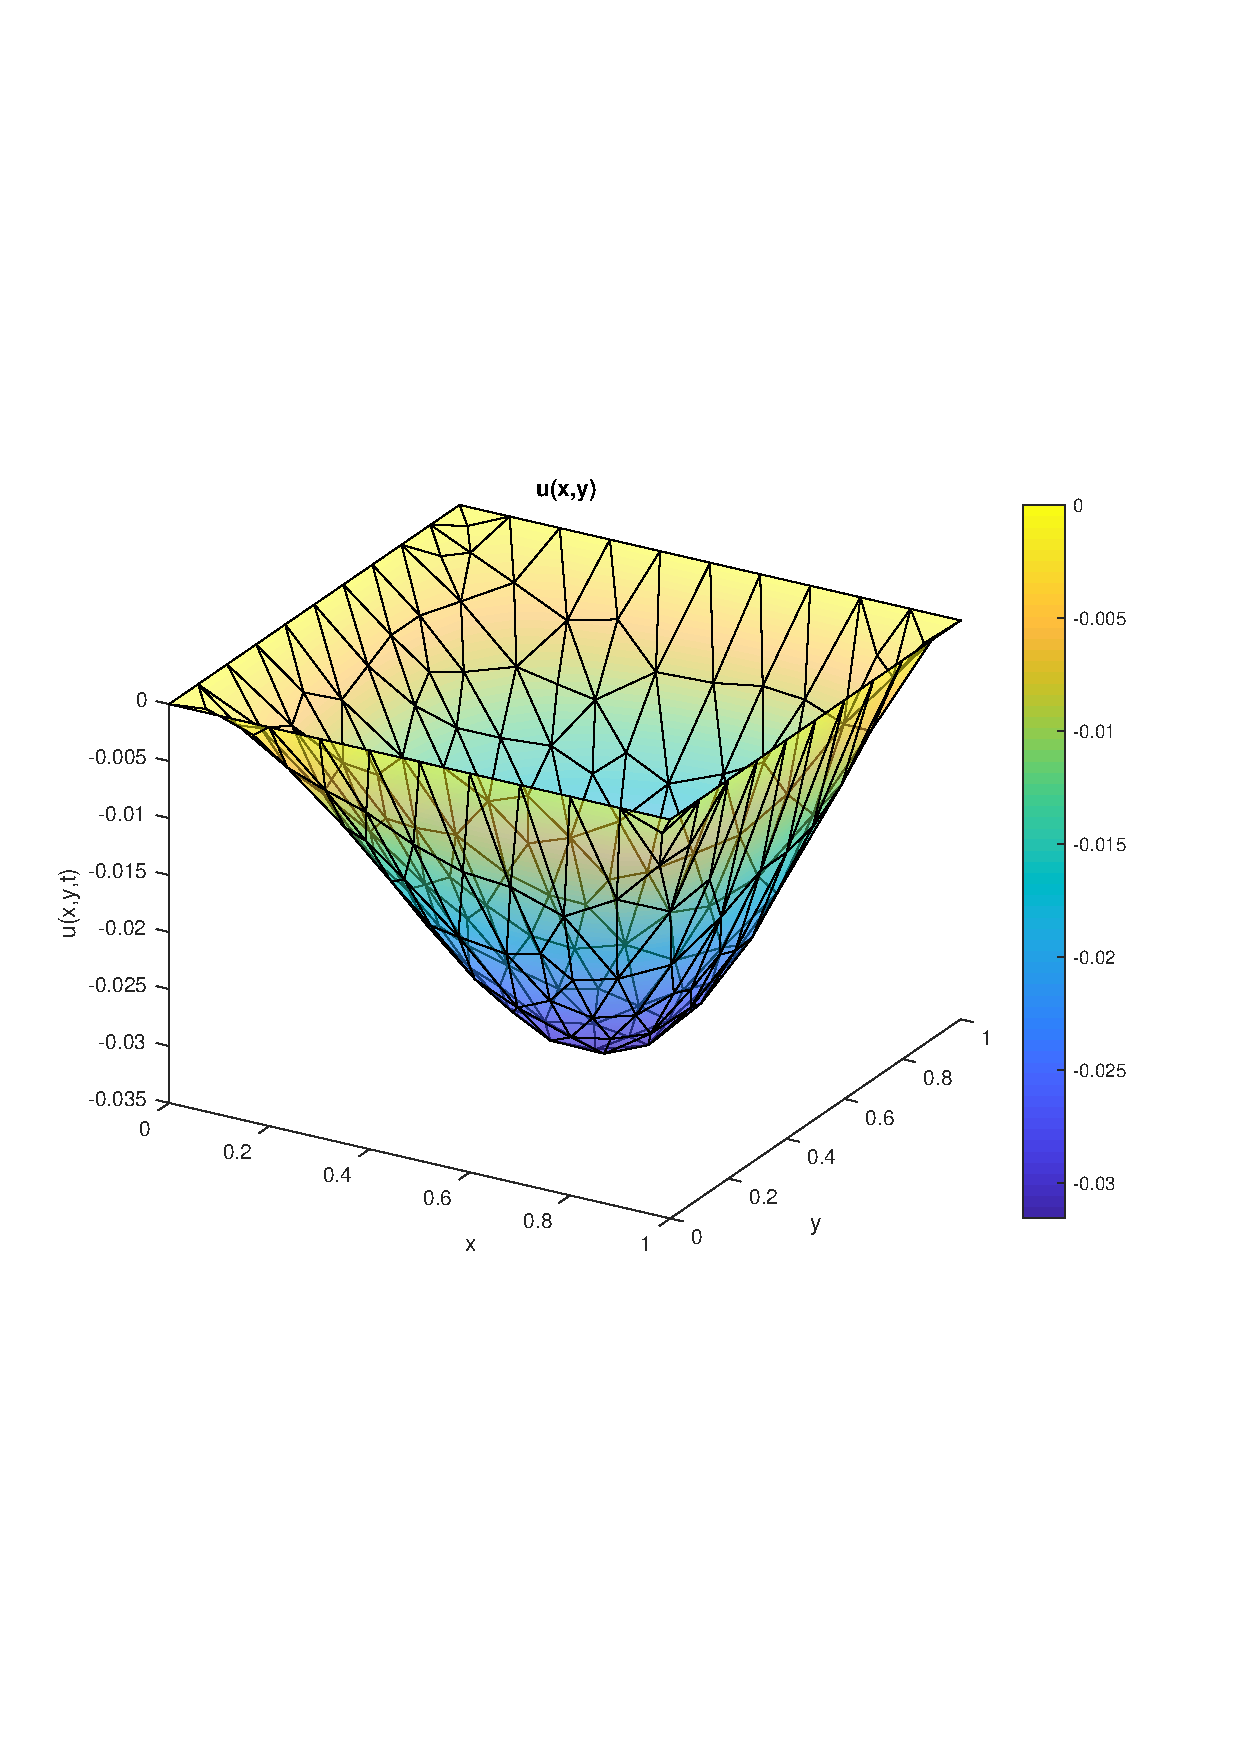
\includegraphics[width=0.49\textwidth]{assets/solution_3d.pdf}
  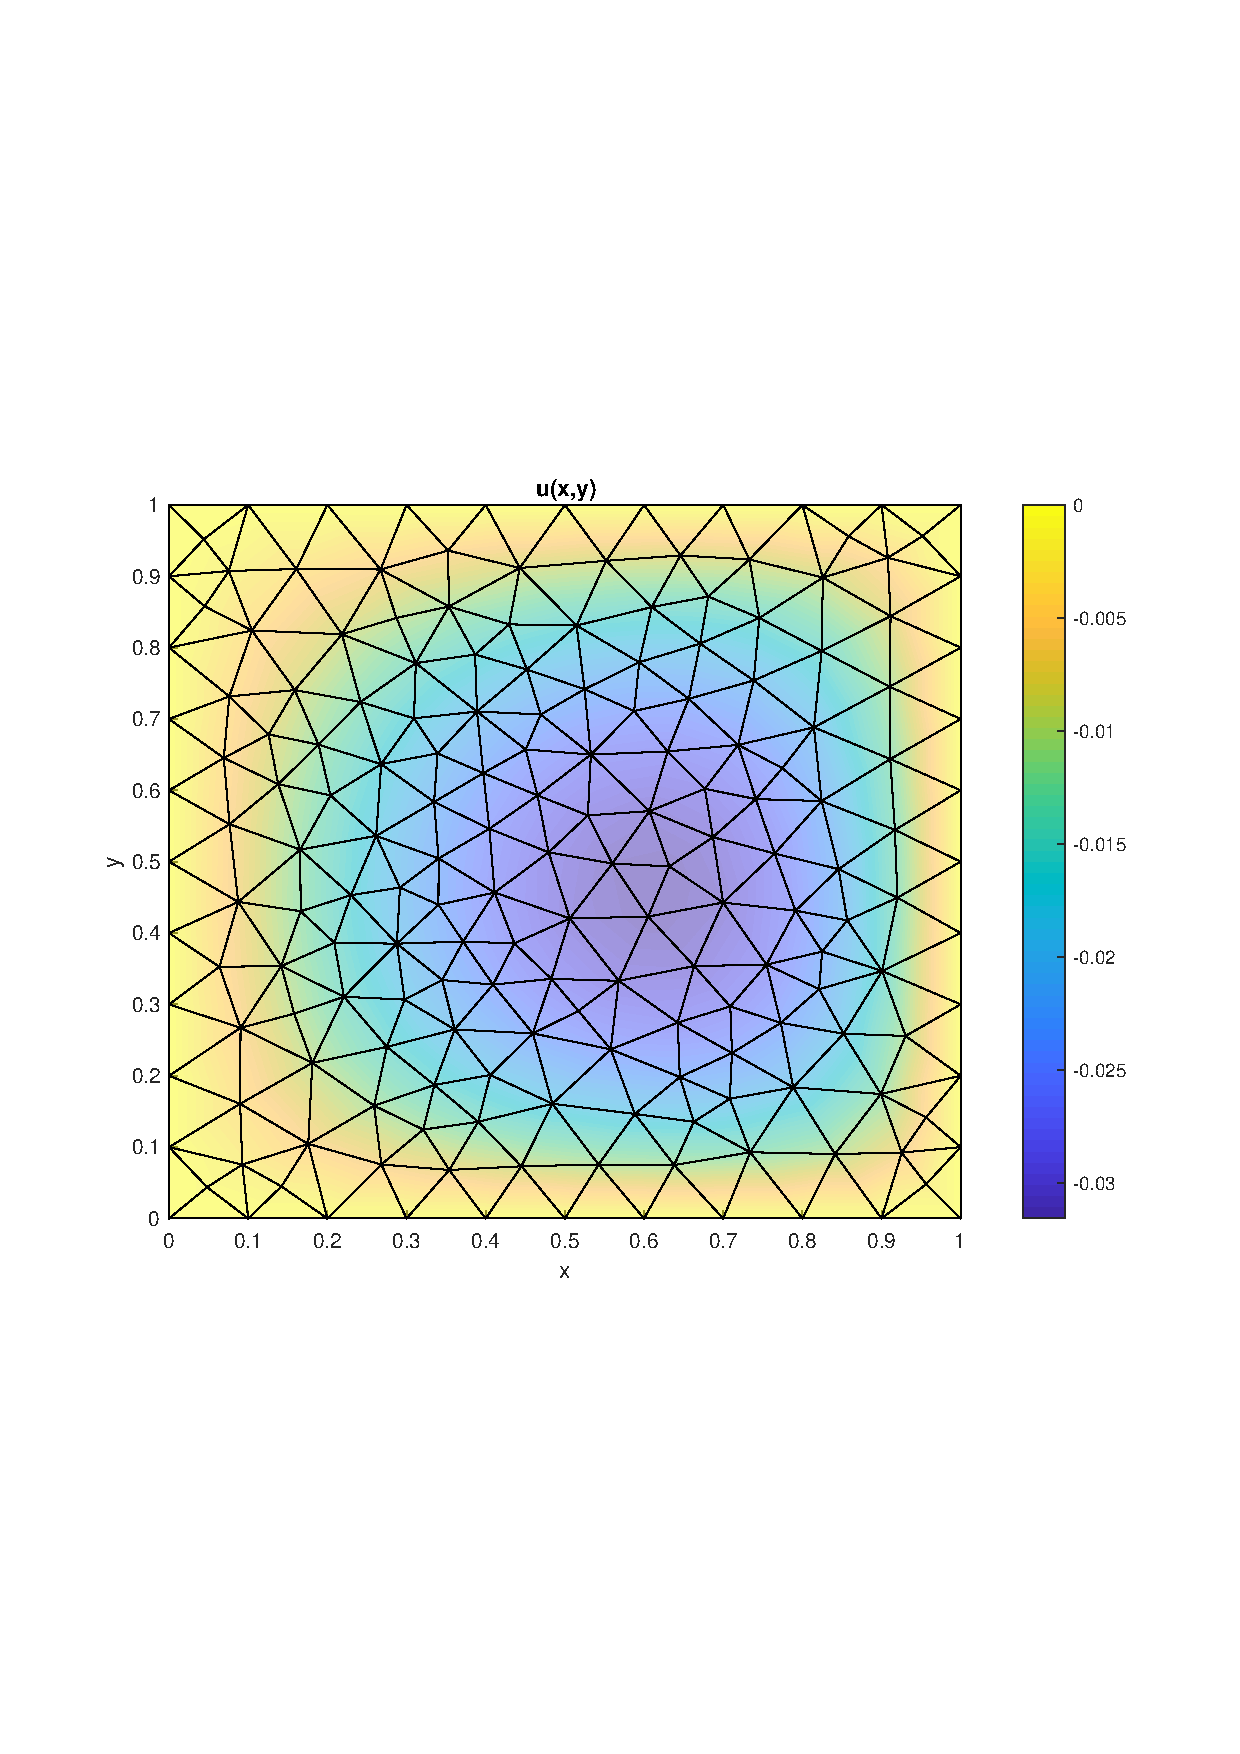
\includegraphics[width=0.49\textwidth]{assets/solution_xy.pdf}
  \caption{Solution $u$ at $t=\infty$}\label{fig:solution}
\end{figure}

\section*{References}
\begin{description}
	\item [(1)] \href{https://github.com/gilbertfrancois/partial-differential-equations/blob/ffee191364d9a2417bef08f517cab05114de68c5/notebook/2D%20Poisson%20equation,%20finite%20difference.ipynb}{Poisson equation, finite difference.ipynb}
	\item [(2)] \href{https://www.mathworks.com/help/releases/R2017a/pde/index.html}{Matlab PDE Toolbox documentation}}
\end{description}
\end{document}
